\documentclass{beamer}

\mode<presentation> {
    \usepackage[utf8]{inputenc}
    \usepackage[T1]{fontenc}
    \usepackage[english]{babel}
    \usepackage{csquotes}
    \usepackage{ragged2e} 
    \usepackage{pgf, tikz}
    \usetikzlibrary{arrows, automata}
    \bibliographystyle{plain}

    \usetheme{Madrid}
    \usecolortheme{ipbutfpr}

    % Can change the colors at beamercolorthemeipbutfpr.sty
    %\setbeamersize{text margin left=0.6cm,text margin right=0.6cm}
    \setbeamertemplate{caption}[numbered]
    \setbeamertemplate{bibliography item}{\insertbiblabel}
    \setbeamertemplate{frametitle continuation}{\gdef\beamer@frametitle{}\justifying}

    \setbeamertemplate{footline}{
        \leavevmode%
        \hbox{%
            \begin{beamercolorbox}[wd=.5\paperwidth,ht=2.25ex,dp=1ex,center]{author in head/foot}%
                \usebeamerfont{author in head/foot}\insertshortauthor
            \end{beamercolorbox}%
            \begin{beamercolorbox}[wd=.5\paperwidth,ht=2.25ex,dp=1ex,center]{title in head/foot}%
                \hspace*{7em}\usebeamerfont{title in head/foot}\insertshorttitle\hspace*{7em}
                \insertframenumber{} / \inserttotalframenumber\hspace*{1ex}
            \end{beamercolorbox}
        }%
        \vskip0pt%
    }

    \setbeamertemplate{navigation symbols}{}
}

\usepackage{amsmath}
\usepackage{amssymb}
\usepackage[language=english, style=numeric, sorting=none]{biblatex}
\usepackage[makeroom]{cancel}

\addbibresource{main.bib}
\makeatletter
\makeatother

\title{\textbf{Graver Basis}}
%\subtitle{A short story}

\author{\textbf{Francisco Javier Blázquez Martínez}}

\institute[EPFL]{\normalsize
    % TODO: How should this be?
    %Project director: Prof. Friedrich Eisenbrand \\
    %Project supervisor: Jana Cslovjecsek \\

    \begin{figure}[htb]
        % TODO: Maybe shift it a little bit to the right
        \centering
        
\includegraphics[width=0.4\textwidth]{images/logos/epfl_logo.png}
    \end{figure}
}

% TODO: Chair of discrete optimization is maybe too much
\date{\small Department of discrete optimization \\ November 2020}

\begin{document}
    \justifying
    
    \frame{\titlepage}
    
    % TODO: Index or not necessary?
    %\begin{frame}
    %\frametitle{Table of Contents}
    %\tableofcontents
    %\end{frame}

    %\begin{frame}
    %\frametitle{Abstract}
    
    %In this presentation we introduce the concept of \textit{Graver basis}, their main properties, bounds, and a general IP algorithm based on these. We also introduce the N-Fold IP as an example of success applying Graver basis related techniques.
    %\end{frame}
    
    \section{Integer Linear Programming}
    \begin{frame}
        \frametitle{Integer Linear Programming}
        \begin{equation*}
            (IP) \equiv max\{c^tx : Ax = b, l \leq x \leq u, x \in \mathbb{Z}^n \}
        \end{equation*}
        \begin{center}
        $A \in \mathbb{Z}^{mxn}$, $b \in \mathbb{Z}^m$, $c \in \mathbb{Z}^n$, $l$  and $u$ lower and upper bounds for x
        \end{center}
        
        %\pause
        % \vspace{1cm}
        % \begin{itemize}
        %     \item NP-Hard
        %     \item Cutting plane methods
        %     \item Lattice-basis reduction
        %     \item Dynamic programming
        %     \item \alert{Graver basis} techniques
        % \end{itemize}
        
        \begin{columns}[T] % align columns
        \begin{column}{.48\textwidth}
        %\color{red}\rule{\linewidth}{4pt}
        %\vspace{0.5cm}
        \begin{itemize}
            \item NP-Hard
            \item Cutting plane methods
            \item Lattice-basis reduction
            \item Dynamic programming
            \item \alert{Graver basis} techniques
        \end{itemize}
        \end{column}%
        \hfill%
        \begin{column}{.48\textwidth}
            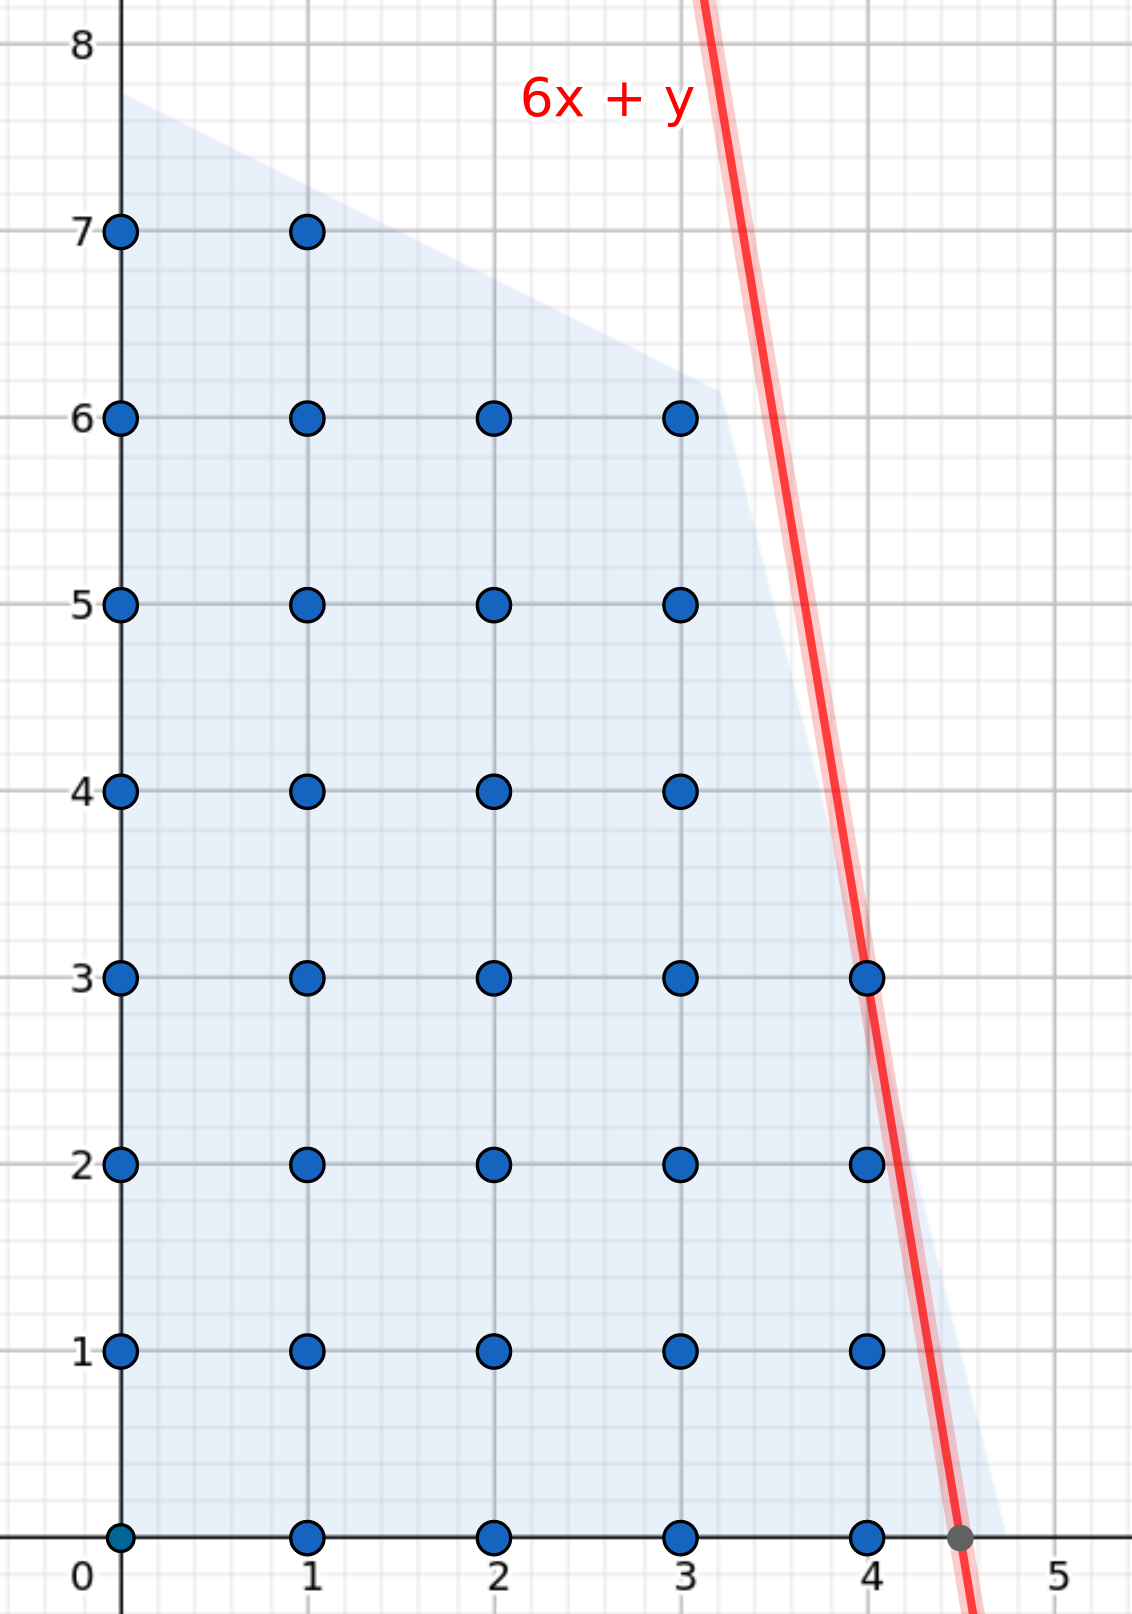
\includegraphics[width=0.6\textwidth]{images/IP(2).png}
        \end{column}%
        \end{columns}
    
        
        % TODO: In case we want to add another column to the slide
        %\begin{columns}[T] % align columns
        %\begin{column}{.48\textwidth}
        %\end{column}
        %\hfill
        %\begin{column}{.48\textwidth}
        %\end{column}%
        %\end{columns}
        
    \end{frame}
    
    % \begin{frame}
    %     \frametitle{Integer Linear Programming}
        
    %     \begin{columns}[T] % align columns
    %     \begin{column}{.48\textwidth}
    %     %\color{red}\rule{\linewidth}{4pt}
    %     \begin{equation*}
    %         (P1) \equiv 	\left( \begin{array}{l}
	   %                     \qquad \max \hspace{2pt}  6x + y  \vspace{4pt} \\ 
	   %                     s.t: 4x + y \leq 19 \\
	   %                     \qquad x + 2y \leq 31 \\
	   %                     \qquad x,y\geq 0 \\
	   %                     \qquad x,y \in \mathbb{Z}
	   %                     \end{array} \right)
    %     \end{equation*}
    %     \end{column}%
    %     \hfill%
    %     \begin{column}{.48\textwidth}
    %         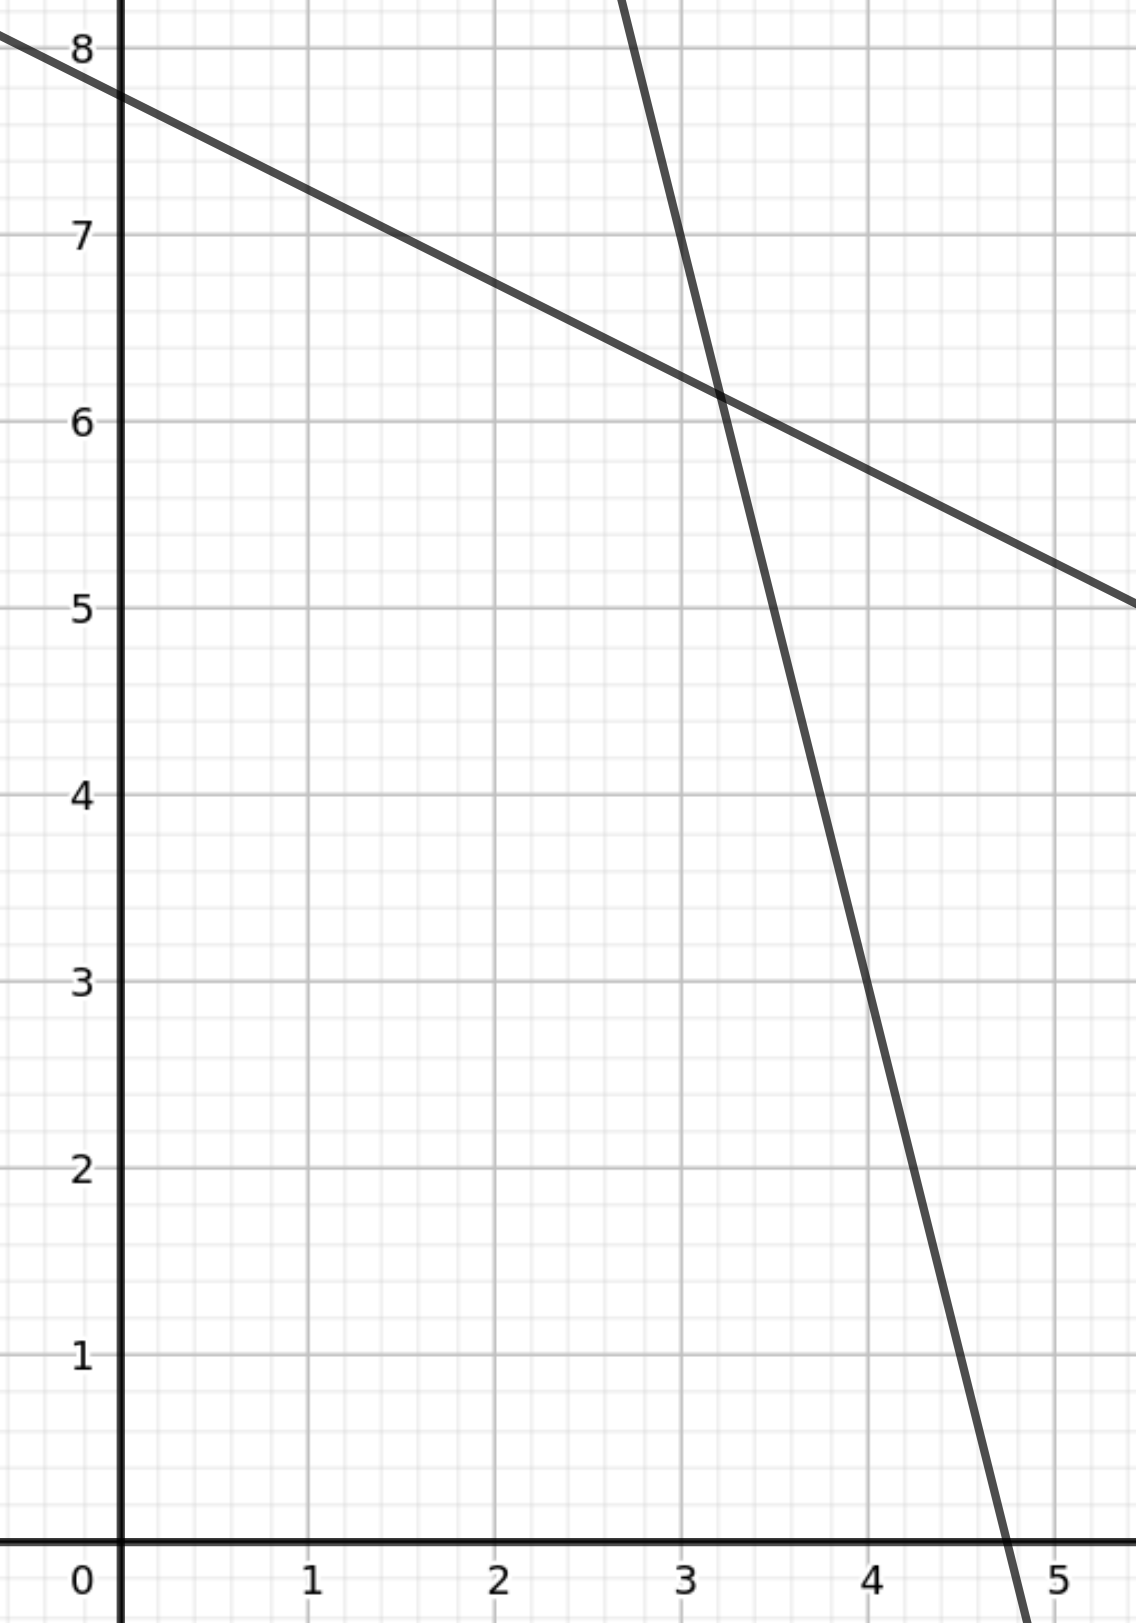
\includegraphics[width=0.85\textwidth]{images/IP(13).png}
    %     \end{column}%
    %     \end{columns}
    %     %\addtocounter{framenumber}{-1}
    % \end{frame}
    
    
    % \begin{frame}
    %     \frametitle{Integer Linear Programming}
        
    %     \begin{columns}[T] % align columns
    %     \begin{column}{.48\textwidth}
    %     %\color{red}\rule{\linewidth}{4pt}
    %     \begin{equation*}
    %         (P1) \equiv 	\left( \begin{array}{l}
	   %                     \qquad \max \hspace{2pt}  6x + y  \vspace{4pt} \\ 
	   %                     s.t: 4x + y \leq 19 \\
	   %                     \qquad x + 2y \leq 31 \\
	   %                     \qquad x,y\geq 0 \\
	   %                     \qquad \xcancel{x,y \in \mathbb{Z}}
	   %                     \end{array} \right)
    %     \end{equation*}
    %     \begin{itemize}
    %         %\item<1-> Text visible on slide 1
    %         %\item<2-> Text visible on slide 2
    %         %\item<3> Text visible on slide 3
    %         %\item<4-> Text visible on slide 4
    %         \item Feasible region
    %         \item Extreme points
    %         \item Extreme directions
    %         \item Optimum in extreme points
    %     \end{itemize}
    %     \end{column}%
    %     \hfill%
    %     \begin{column}{.48\textwidth}
    %         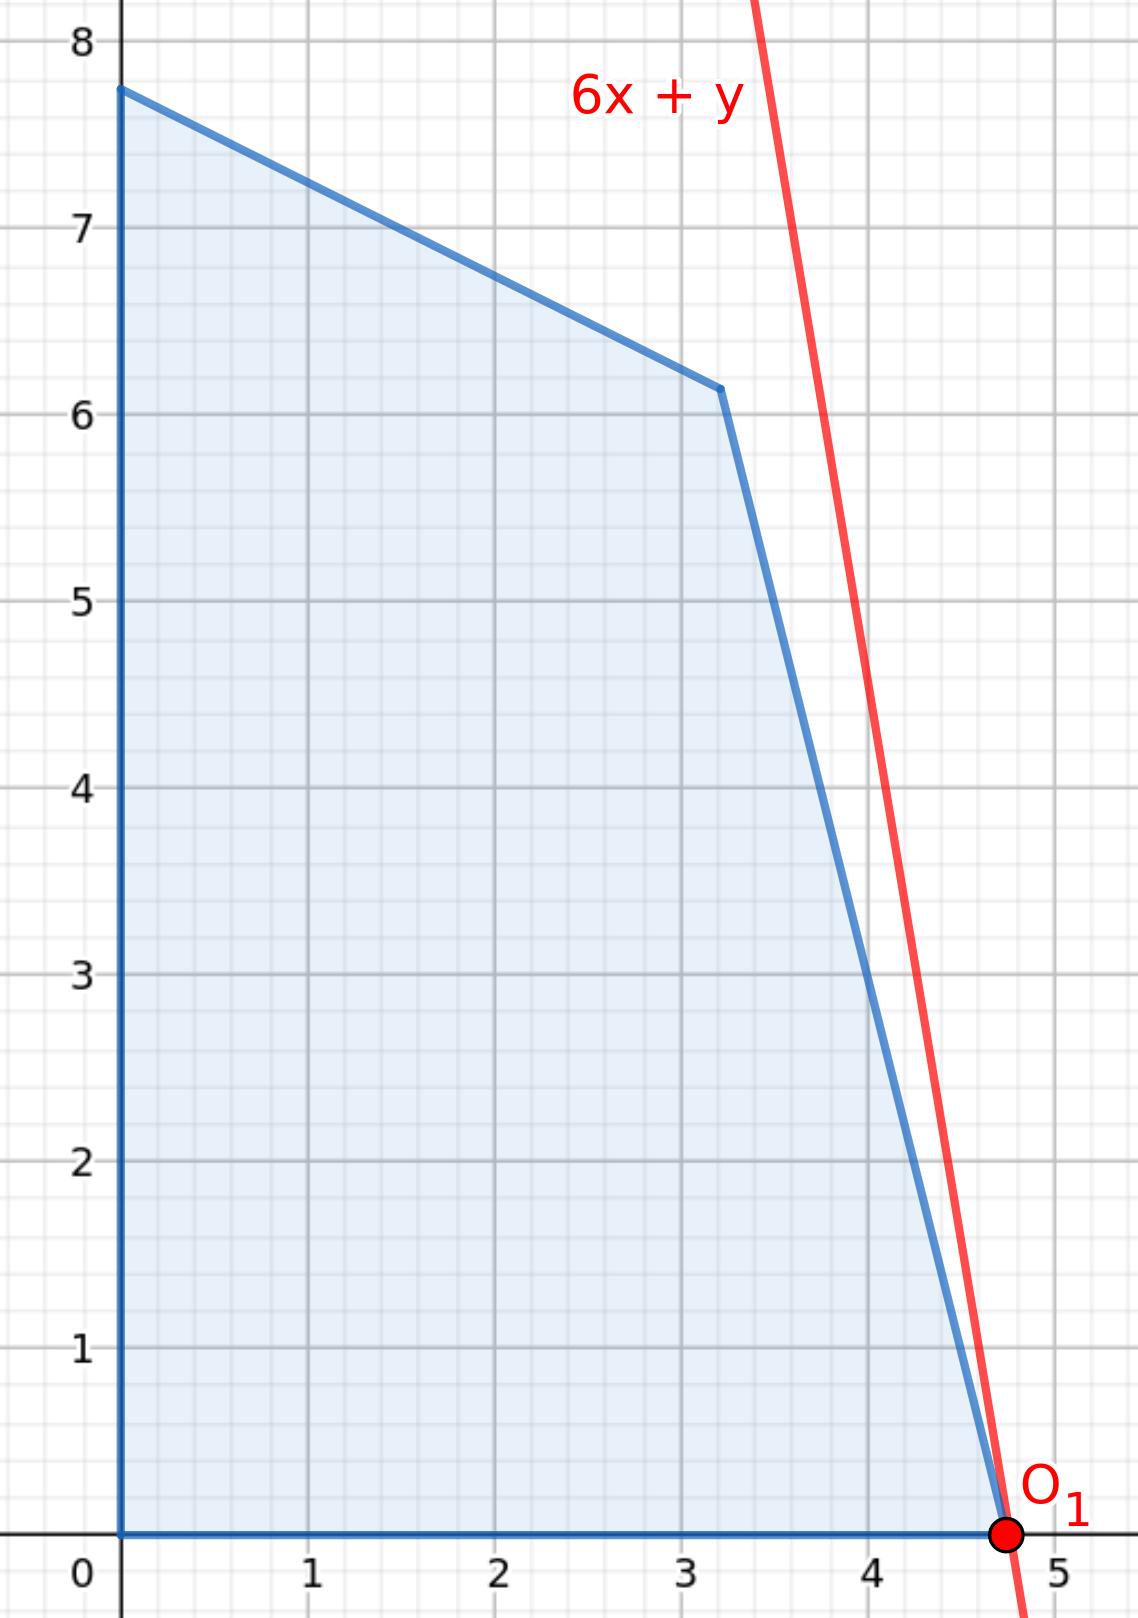
\includegraphics[width=0.85\textwidth]{images/IP(3).png}
    %     \end{column}%
    %     \end{columns}
        
    %     \addtocounter{framenumber}{-1}

    % \end{frame}
    
    %     \begin{frame}
    %     \frametitle{Integer Linear Programming}
        
    %     \begin{columns}[T] % align columns
    %     \begin{column}{.48\textwidth}
    %     %\color{red}\rule{\linewidth}{4pt}
    %     \begin{equation*}
    %         (P1) \equiv 	\left( \begin{array}{l}
	   %                     \qquad \max \hspace{2pt}  6x + y  \vspace{4pt} \\ 
	   %                     s.t: 4x + y \leq 19 \\
	   %                     \qquad x + 2y \leq 31 \\
	   %                     \qquad x,y\geq 0 \\
	   %                     \qquad x,y \in \mathbb{Z}
	   %                     \end{array} \right)
    %     \end{equation*}
    %     \begin{itemize}
    %         \item Feasible points
    %         \item Optimum can be far from the linear relaxation solution.
    %     \end{itemize}
    %     \end{column}%
    %     \hfill%
    %     \begin{column}{.48\textwidth}
    %         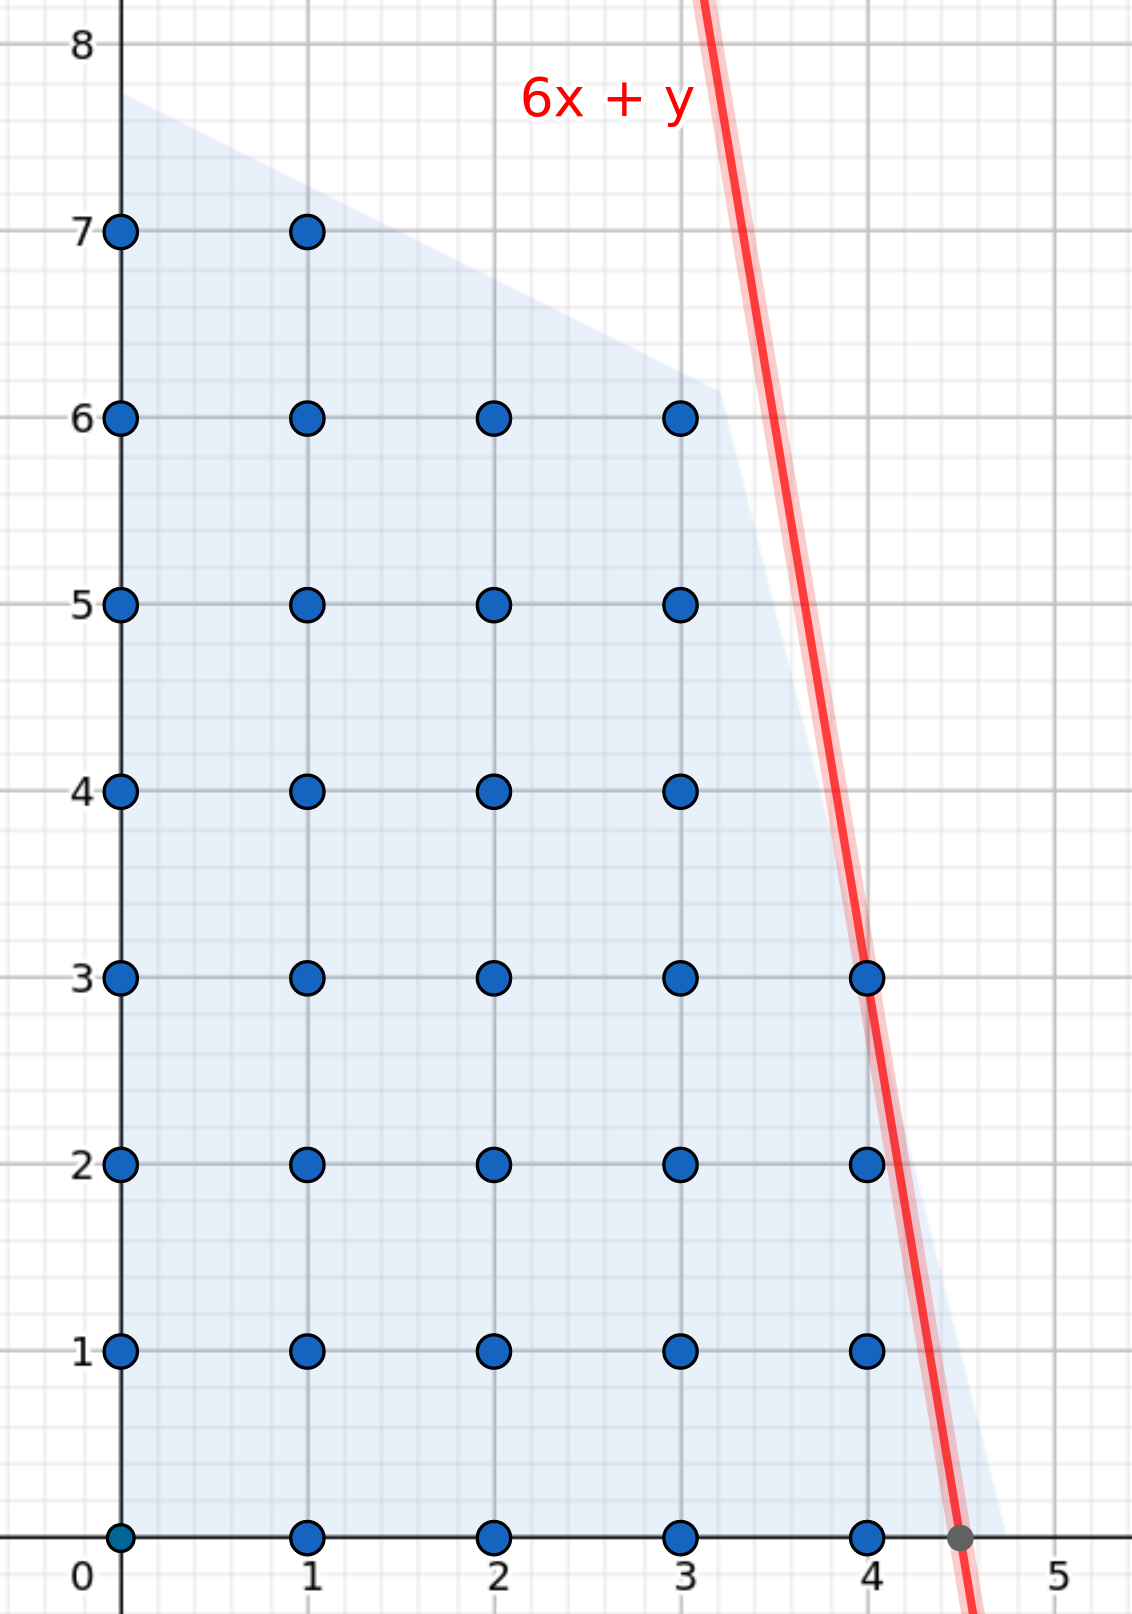
\includegraphics[width=0.85\textwidth]{images/IP(2).png}
    %     \end{column}%
    %     \end{columns}
        
    %     \addtocounter{framenumber}{-1}

    % \end{frame}
    
    %     \begin{frame}
    %     \frametitle{Integer Linear Programming}
        
    %     \begin{columns}[T] % align columns
    %     \begin{column}{.48\textwidth}
    %     %\color{red}\rule{\linewidth}{4pt}
    %     \begin{equation*}
    %         (P1) \equiv 	\left( \begin{array}{l}
	   %                     \qquad \max \hspace{2pt}  6x + y  \vspace{4pt} \\ 
	   %                     s.t: 4x + y \leq 19 \\
	   %                     \qquad x + 2y \leq 31 \\
	   %                     \qquad x,y\geq 0 \\
	   %                     \qquad \xcancel{x,y \in \mathbb{Z}}
	   %                     \end{array} \right)
    %     \end{equation*}
    %     \begin{itemize}
    %         %\item<1-> Text visible on slide 1
    %         %\item<2-> Text visible on slide 2
    %         %\item<3> Text visible on slide 3
    %         %\item<4-> Text visible on slide 4
    %         \item Extreme directions: \\
    %         Allow Simplex fast optimality test and finding a direction of improvement in LP. 
            
    %         \vspace{0.5cm}
    %         Can we do the same for IP?
    %     \end{itemize}
    %     \end{column}%
    %     \hfill%
    %     \begin{column}{.48\textwidth}
    %         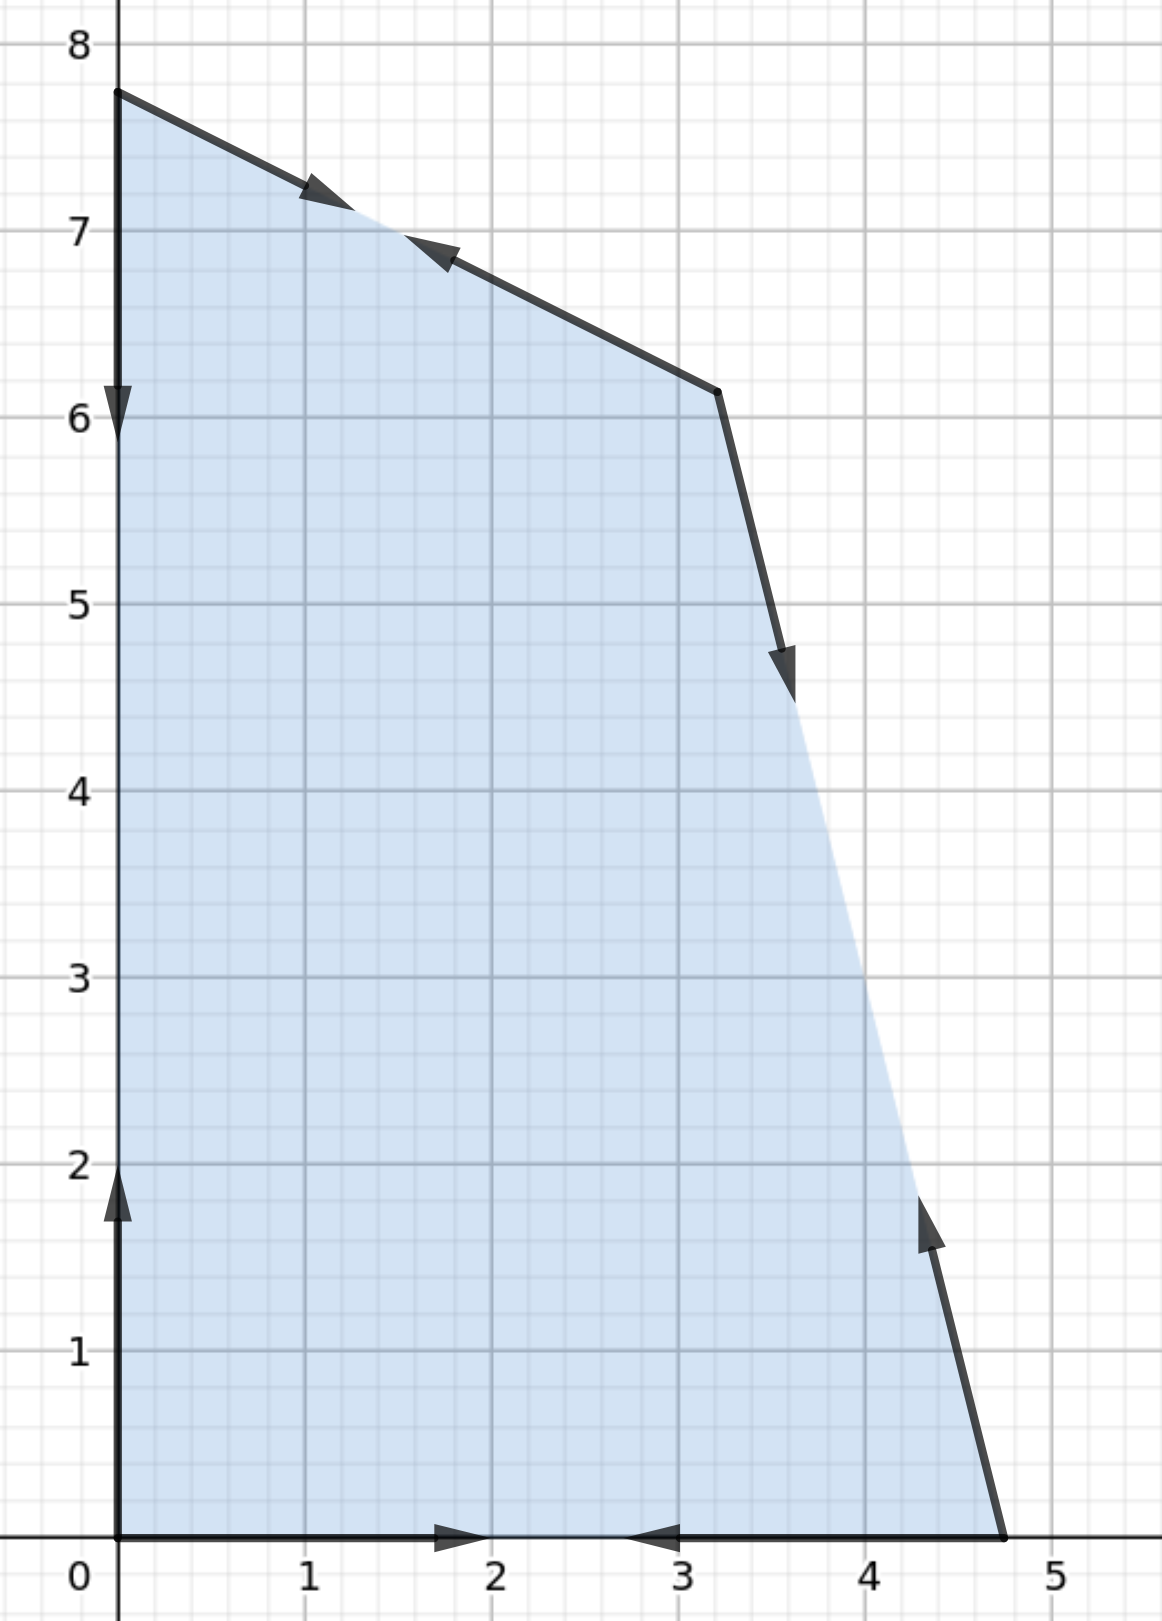
\includegraphics[width=0.85\textwidth]{images/IP(4).png}
    %     \end{column}%
    %     \end{columns}
        
    %     \addtocounter{framenumber}{-1}

    % \end{frame}

    \section{Graver Basis, definition and properties}
    \begin{frame}
        \frametitle{Graver Basis}
        \begin{itemize}
            \item \textbf{Definition:} Two vectors $u,v \in \mathbb{R}^n$ are said to be \textbf{sign compatible} if $u_i \cdot v_i \geq 0$ for all $i \in \{1,...,n\}$
            \vspace{0.2cm}
            %\pause
            \item \textbf{Definition:} A vector $u \in ker(A)$ is \textbf{indecomposable} if it is not the sum of two sign compatible and non zero elements in $ker(A)$.
            %\pause
        \end{itemize}
        
        %\pause
        \vspace{1cm}
        \begin{block}{Graver Basis $\equiv Gr(A)$ }
            The Graver Basis of a given matrix A is defined as the set of integral indecomposable elements in the kernel of A.
        \end{block}
        (Initially defined as \textit{universal integral test set} in [Graver 1975])
    \end{frame}
    
    \begin{frame}
        \frametitle{Graver Basis properties}
        \begin{itemize}
            \justifying
            \item \textbf{Spanning:} Every integral element in ker(A) can be expressed as positive integral linear combination of elements in $Gr(A)$.
        \end{itemize}
        
        \vspace{0.5cm}
        \begin{itemize}
            \justifying
            \item \textbf{Optimality:} Given z in the feasible region of an IP, z is not optimum if and only if there exists $g \in Gr(A)$ s.t. $c^tg > 0$ and $l \leq z + g \leq u$
            %\pause
        \end{itemize}
        
        
        %\pause
        \vspace{0.5cm}
        \begin{itemize}
            \justifying
            \item \textbf{Bounds:} Given $A \in \mathbb{Z}^{mxn}$ and $\Delta$ an upper bound for the absolute value of each component of $A$, for every $g \in Gr(A)$:
            \begin{itemize}
                \item $||g||_1 \leq m^{m/2}\Delta^m\cdot(n - m)$ \hspace{10pt}[Onn 2010]
                \item $||g||_1 \leq (2m \Delta + 1)^m$ \hspace{35pt}[Eisenbrand,Hunkenschröder,Klein 2018]
            \end{itemize}
            %\pause
        \end{itemize}

        
    \end{frame}
    
    \begin{frame}
        \frametitle{Graver Basis properties}
        
        \begin{columns}[T] % align columns
        \begin{column}{.48\textwidth}
        %\color{red}\rule{\linewidth}{4pt}
        \begin{equation*}
            (P1) \equiv 	\left( \begin{array}{l}
	                        \qquad \max \hspace{2pt}  6x + y  \vspace{4pt} \\ 
	                        s.t: 4x + y \leq 19 \\
	                        \qquad x + 2y \leq 31 \\
	                        \qquad x,y\geq 0 \\
	                        \qquad x,y \in \mathbb{Z}
	                        \end{array} \right)
        \end{equation*}
        \begin{itemize}
            \justifying
            %\item<1-> Text visible on slide 1
            %\item<2-> Text visible on slide 2
            %\item<3> Text visible on slide 3
            %\item<4-> Text visible on slide 4
            \item If not optimal, an element in Graver basis is an improvement direction.
            \item If Graver basis bounded, we can restrict our improvement direction search.
        \end{itemize}
        \end{column}%
        \hfill%
        \begin{column}{.48\textwidth}
            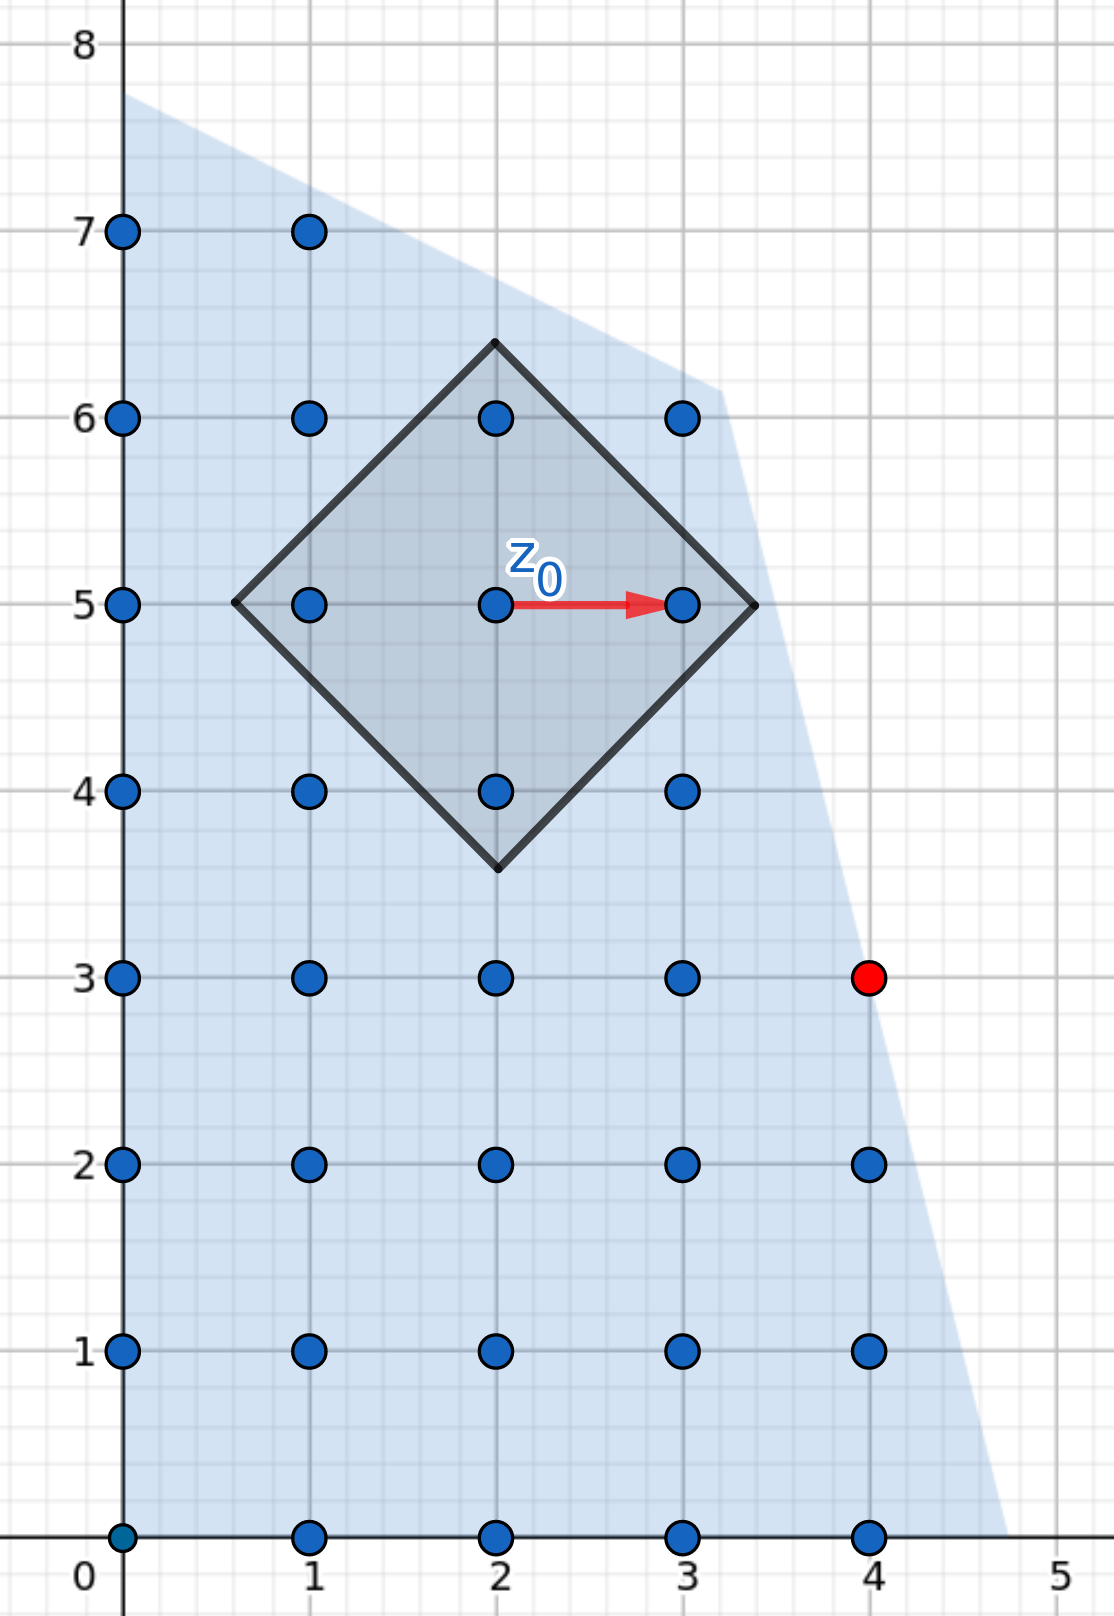
\includegraphics[width=0.85\textwidth]{images/IP(6).png}
        \end{column}%
        \end{columns}
    \end{frame}
    
    \begin{frame}
        \frametitle{Augmentation algorithm}
        %The following is a general IP algorithm. At first sight it may not seem an improvement, however, in the sub-problem the feasible region is being restricted to elements bounded by Graver basis norm, which reduces the problem considerably in certain cases. 

        %\vspace{0.5cm}
        %The correctness of this algorithm is given by \textbf{property 2}. 
        %\vspace{0.5cm}
        \begin{block}{\centering General IP algorithm using Graver basis norm bound}
        \begin{enumerate}
            \item From a feasible solution $z_i$
            \item Find $g^*$ optimum for the sub-problem: \vspace{4pt}\\
                  $max\{c^tg : Ag = 0, l-z_i \leq g \leq u-z_i, g \in \mathbb{Z}^n, ||g||_1 \leq ||Gr(A)|| \}$ \vspace{4pt}
            \begin{itemize}
                \item $g^* = 0 \implies z_i$ optimal solution.
                \item $g^* \neq 0 \implies$ $g^*$ improvement direction, loop back to 1 with $z_{i+1} = z_i + \lambda \cdot g^*$ with the biggest $\lambda$ respecting the bounds.
            \end{itemize}
        \end{enumerate}
        \end{block}
        [Hemmecke, Onn, Romanchuk 2013]
    \end{frame}
    
    \section{N-Fold, a success example}
    \begin{frame}
        \frametitle{N-Fold, a success example}
        
        A N-Fold IP has constriction matrix A of the form ($A_i \in \mathbb{Z}^{rxt}, B_i \in \mathbb{Z}^{sxt}$):\\
        \begin{equation*}
        N = 
        \begin{pmatrix}
        A_1 & A_2 & \cdots & A_n \\
        B_1 & 0   & \cdots & 0 \\
        0   & B_2 & \cdots & 0 \\
        \vdots    & \vdots & \ddots & \vdots  \\
        0   & 0   & \cdots & B_n 
        \end{pmatrix}
        \end{equation*}
        
        %\vspace{0.5cm}
        %It's possible (using Steinitz Lemma) to obtain a much tighter bound for the norm of the elements in the Graver basis than the ones mentioned before.
        
        %\pause
        \begin{block}{N-Fold Graver basis bound}
            For all $g \in Gr(N)$ $||g||_1 \leq L_B (2r\Delta L_B + 1)^r =: L_A$ where $L_B = (2s \Delta + 1)^s$
        \end{block}
        %\pause
        \begin{block}{N-Fold augmentation algorithm complexity}
            The N-Fold IP can be solved in time $(nt)^2 log^2(nt) \cdot \varphi (rs\Delta)^{O(r^2s + rs^2)} + LP$
        \end{block}
        %\addtocounter{framenumber}{-1}
        
        [Eisenbrand, Hunkenschröder, Klein 2018]
    \end{frame}
    
    \begin{frame}
        \frametitle{N-Fold, improving even more}
        
        \begin{figure}[!tbp]
        \centering
        \begin{minipage}[b]{0.45\textwidth}
            \centering
            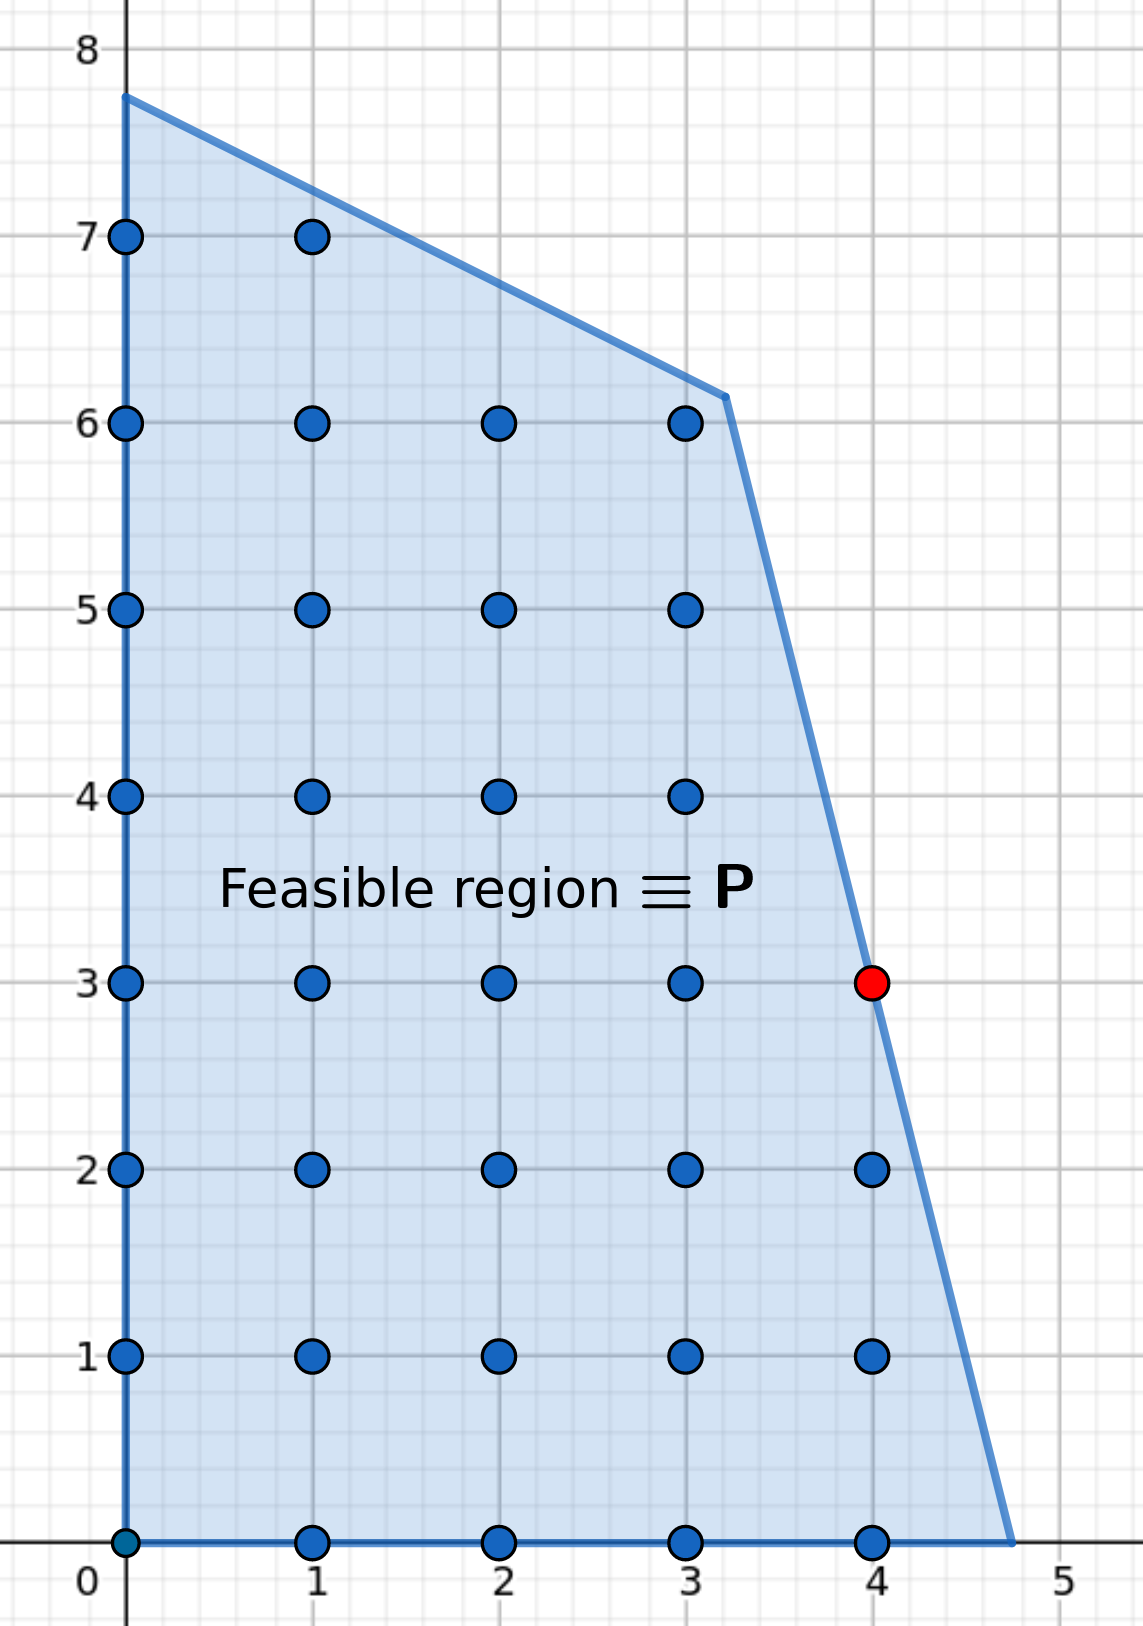
\includegraphics[width=0.9\textwidth]{images/IP(12).png}
            \caption{Linear Relaxation (LR)}
        \end{minipage}
        \hfill
        \begin{minipage}[b]{0.45\textwidth}
            \centering
            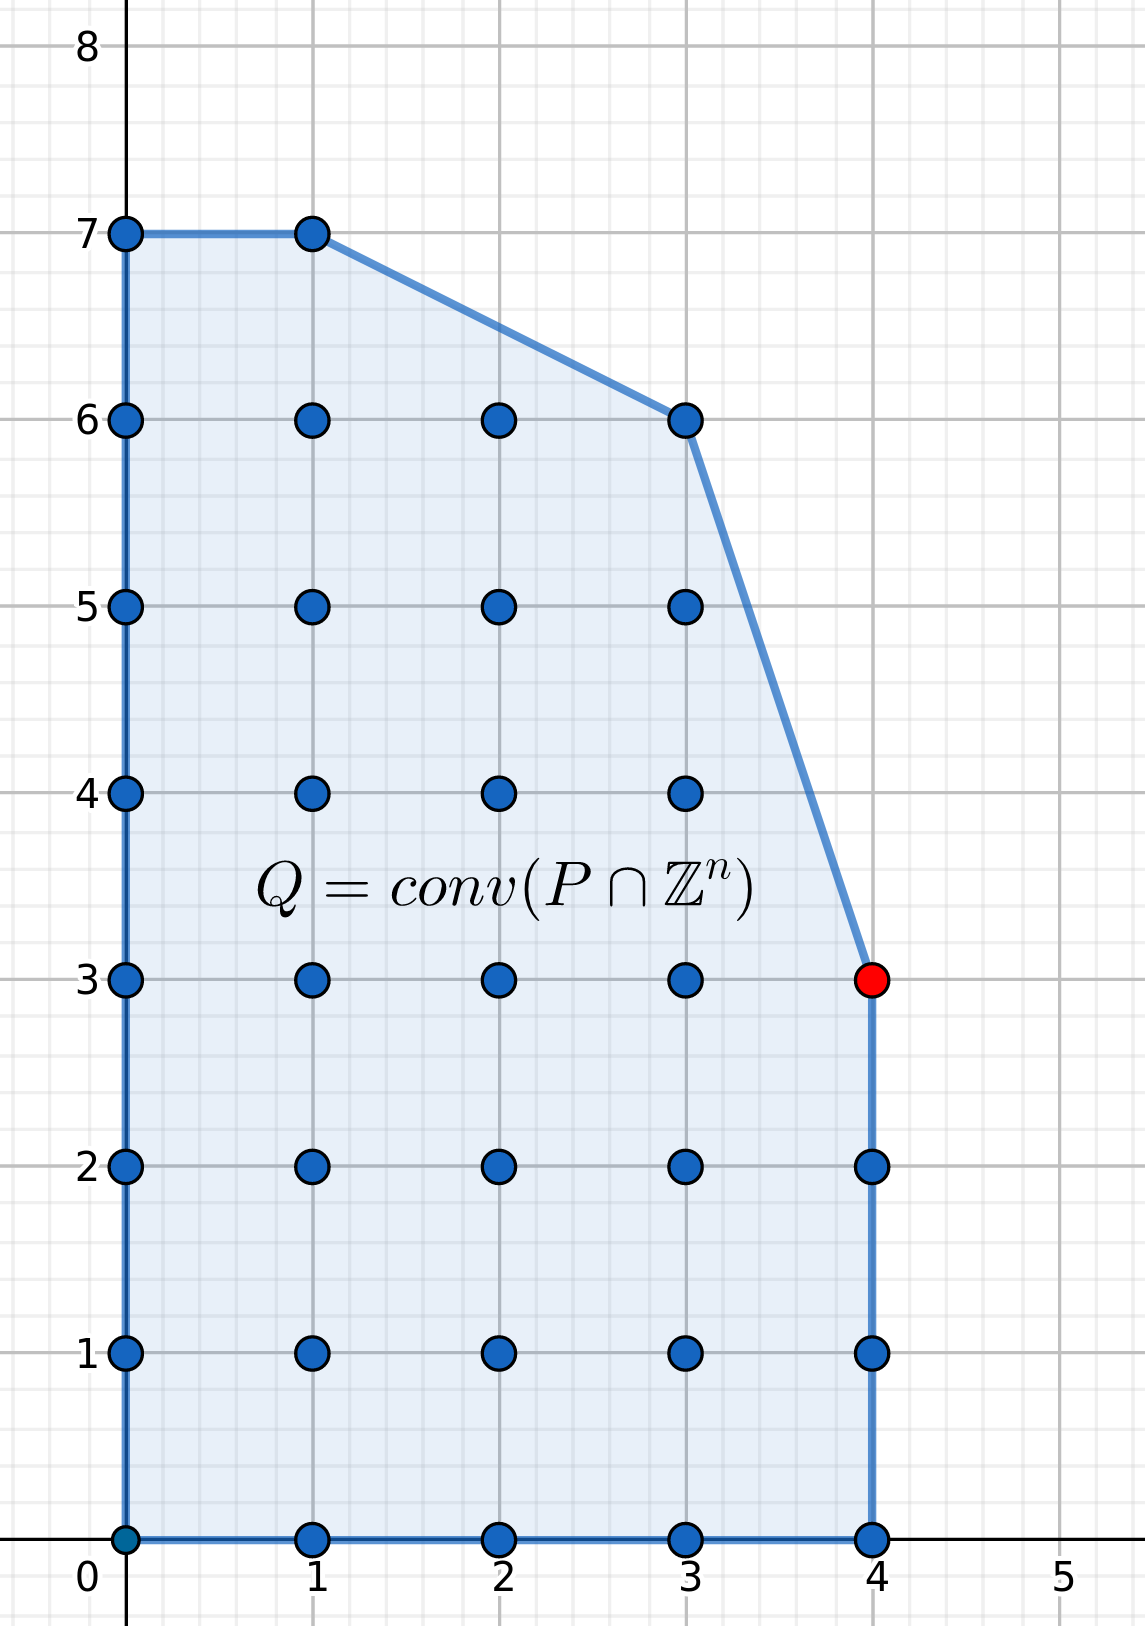
\includegraphics[width=0.9\textwidth]{images/IP(10).png}
            \caption{Restricted LR (RLR)}
        \end{minipage}
        \end{figure}
    \end{frame}
    \begin{frame}
        \frametitle{N-Fold, resolution steps}
        % TODO: RLR might not be the best notation
        \begin{block}{N-Fold RLR complexity}
            The N-Fold IP restricted linear relaxation problem can be solved in time
            \begin{equation*}
                % TODO: Can be more beautiful!
                O(nt \cdot log^2(nt) \cdot \varphi p(r) (s\Delta)^{O(s^2)})
            \end{equation*}
        \end{block}
        \vspace{0.5cm}
        % TODO: Fill this block properly!
        \begin{block}{N-Fold RLR to optimum complexity}
            Given an optimal vertex of an N-Fold RLR, the N-Fold IP can be solved in time
            \begin{equation*}
                O(nt \cdot (rs\Delta)^{O(r^2s+s^2)})
            \end{equation*}
        \end{block}
        [Cslovjecsek, Eisenbrand, Weismantel 2020]
    \end{frame}
    \begin{frame}
        \frametitle{N-Fold, from RLR to optimum}
        \begin{block}{N-Fold proximity to RLR}
            Let $x^*$ be an optimal vertex solution of a N-Fold RLR, then there exists an optimal solution $z^*$ for the N-Fold IP verifying:  
            \begin{equation*}
                ||z^* - x^*||_1 \leq (rs\Delta)^{O(rs)}
            \end{equation*}
        \end{block}
        [Cslovjecsek, Eisenbrand, Weismantel 2020]
        \vspace{0.5cm}
        
        Let $\gamma := (rs\Delta)^{O(rs)}$. For every $1 \leq \ell \leq n$:
        \vspace{-0.25cm}
        \begin{align*}
            ||x^* - z||_1 \leq \gamma 
            & \implies \sum_{i=1}^\ell ||x_i^* - z_i||_1 \leq \gamma\\ 
            & \implies \sum_{i=1}^\ell ||A_i(x_i^* - z_i)||_\infty \leq \Delta \gamma = \gamma
        \end{align*}
        % Therefore for all $1 \leq l \leq n$ we have that:
        % \begin{align*}
        %     % \forall 1 \leq l \leq n
        %     \sum_{i=0}^l ||A_i(x^* - z^*)||_\infty 
        %     & \leq s\Delta \sum_{i=0}^l ||x^* - z^*||_\infty \\
        %     & \leq s\Delta \sum_{i=0}^n ||x^* - z^*||_\infty \\
        %     & \leq s\Delta (rs\Delta)^{O(rs)} = (rs\Delta)^{O(rs)}
        % \end{align*}
        
    \end{frame}
    \begin{frame}
        \frametitle{N-Fold, from RLR to optimum}
        Therefore, for every feasible point z verifying the proximity bound we have:
        \begin{equation*}
            % \forall 1 \leq l \leq n
            \sum_{i=1}^\ell A_ix_i^* - \gamma \leq \sum_{i=1}^\ell A_iz_i \leq \sum_{i=1}^\ell A_ix_i^* + \gamma 
            %& \leq s\Delta \sum_{i=0}^l ||x^* - z^*||_\infty \\
            %& \leq s\Delta \sum_{i=0}^n ||x^* - z^*||_\infty \\
            %& \leq s\Delta (rs\Delta)^{O(rs)} = (rs\Delta)^{O(rs)}
        \end{equation*}
        
        We now define the set $S_\ell$ as the set of $y \in \mathbb{Z}^r$ such that:
        \begin{equation*}
        \sum_{i=1}^\ell A_ix_i^* - \gamma \leq y \leq \sum_{i=1}^\ell A_ix_i^* + \gamma 
        \end{equation*}
        
        % TODO: Uncomment if able to get the |E| bound
        %\vspace{0.1cm}
        %It's clear that $|S_\ell| \leq O(\gamma^r) = (rs\Delta)^{O(r^2s)}$
        
        % \begin{itemize}
        %     \item $|S_l| \leq (rs\Delta)^{O(r^2s)}$
        %     \item $ \sum_{i=1}^\ell A_iz_i \in S_\ell $ $\forall 1 \leq \ell \leq n$, z feasible point in the proximity bound 
        %     \item The last point includes also at least one optimal solution $z^*$
        % \end{itemize}
        
        %TODO: Replace z* in the inequalities by z and explain that z* is there
        
        %And the idea is that we can pose the problem of finding $z^*$ as a longest path problem in a weighted directed acyclic graph. 
        
    \end{frame}
    \begin{frame}{N-Fold, from RLR to optimum}
        % TODO: Graph, correspondence theorem, proof!
        We can construct a weighted directed acyclic graph G(V,E) with vertices:
        \begin{equation*}
            V = \{(\ell,y) / y \in S_\ell\} \cup \{ (0,0), (n,b_0) \}
        \end{equation*}
        \vspace{1.5mm}
        
        \begin{center}
    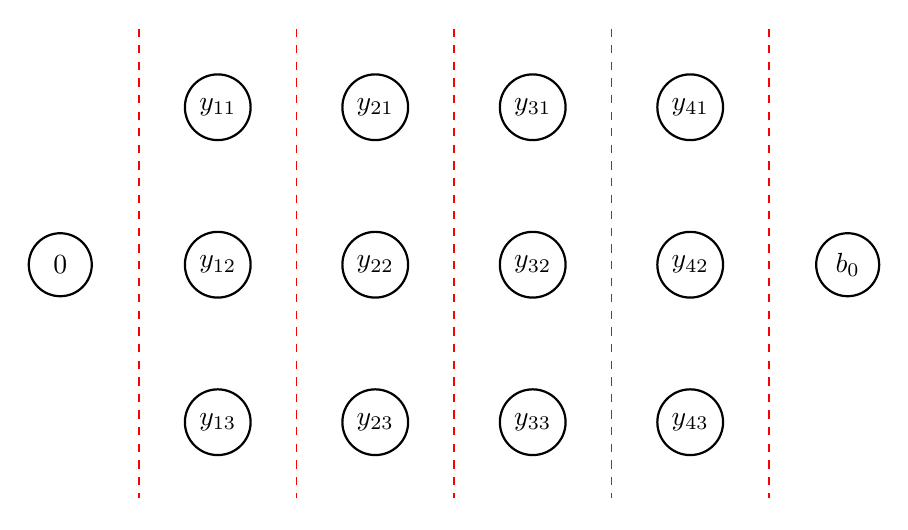
\begin{tikzpicture}[
            > = stealth, % arrow head style
            shorten > = 1pt, % don't touch arrow head to node
            auto,
            node distance = 3cm, % distance between nodes
            semithick % line style
        ]

        \tikzstyle{every state}=[
            draw = black,
            thick,
            fill = white,
            minimum size = 4mm
        ]

        \node[state, minimum size=0.8cm] (s) at (0,0) {$0$};
        
        \node[state] (w1) at (2,2)  {$y_{11}$};
        \node[state] (u1) at (2,0)  {$y_{12}$};
        \node[state] (v1) at (2,-2) {$y_{13}$};
        
        %\node (u2) at (4,0)  {$\sum_{i=1}^\ell A_ix^*$};
        \node[state] (w2) at (4,2)  {$y_{21}$};
        \node[state] (u2) at (4,0)  {$y_{22}$};
        \node[state] (v2) at (4,-2) {$y_{23}$};
        
        \node[state] (w3) at (6,2)  {$y_{31}$};
        \node[state] (u3) at (6,0)  {$y_{32}$};
        \node[state] (v3) at (6,-2) {$y_{33}$};
        
        \node[state] (w4) at (8,2)  {$y_{41}$};
        \node[state] (u4) at (8,0)  {$y_{42}$};
        \node[state] (v4) at (8,-2) {$y_{43}$};
        
        \node[state, minimum size=0.8cm] (f) at (10,0)  {$b_0$};
        
        \draw[red, dashed] (1, 3) -- (1, -3);
        \draw[red, dashed] (3, 3) -- (3, -3);
        \draw[red, dashed] (5, 3) -- (5, -3);
        \draw[red, dashed] (7, 3) -- (7, -3);
        \draw[red, dashed] (9, 3) -- (9, -3);
        
        % \node (S1) at (2,-3.5) {$S_1$};
        % \node (S2) at (4,-3.5) {$S_2$};
        % \node (S3) at (6,-3.5) {$S_3$};
        % \node (S4) at (8,-3.5) {$S_4$};
    \end{tikzpicture}
    \end{center}
    \addtocounter{framenumber}{-1}
    \end{frame}
    \begin{frame}{N-Fold, from RLR to optimum}
        Weighted edges between $(\ell-1,y)$ and $(\ell,y')$ if the problem is feasible:
        \begin{equation*}
            max\{c_\ell^tx: A_\ell x = (y'-y), B_\ell x = b_\ell, l_\ell \leq x \leq u_\ell \}
        \end{equation*}
        \vspace{1.5mm}
        
                \begin{center}
    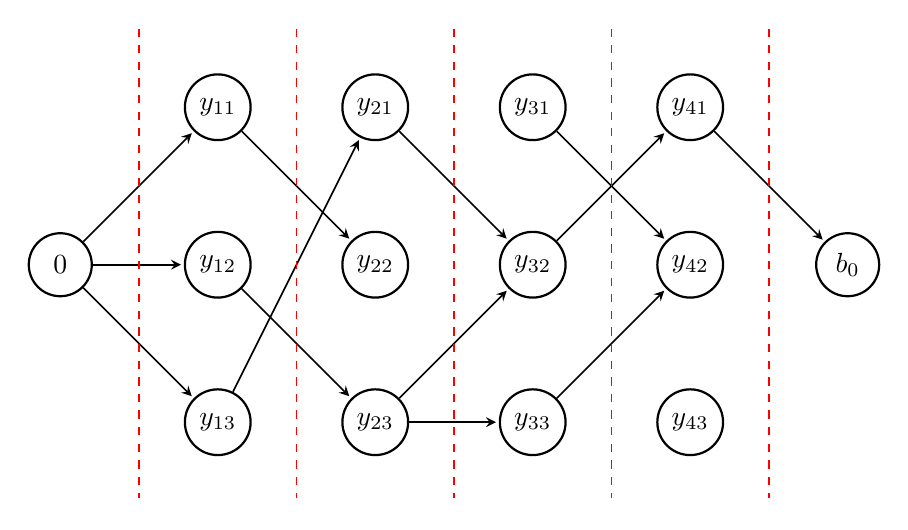
\begin{tikzpicture}[
            > = stealth, % arrow head style
            shorten > = 1pt, % don't touch arrow head to node
            auto,
            node distance = 3cm, % distance between nodes
            semithick % line style
        ]

        \tikzstyle{every state}=[
            draw = black,
            thick,
            fill = white,
            minimum size = 4mm
        ]

        \node[state, minimum size=0.8cm] (s) at (0,0) {$0$};
        
        \node[state] (w1) at (2,2)  {$y_{11}$};
        \node[state] (u1) at (2,0)  {$y_{12}$};
        \node[state] (v1) at (2,-2) {$y_{13}$};
        
        %\node (u2) at (4,0)  {$\sum_{i=1}^\ell A_ix^*$};
        \node[state] (w2) at (4,2)  {$y_{21}$};
        \node[state] (u2) at (4,0)  {$y_{22}$};
        \node[state] (v2) at (4,-2) {$y_{23}$};
        
        \node[state] (w3) at (6,2)  {$y_{31}$};
        \node[state] (u3) at (6,0)  {$y_{32}$};
        \node[state] (v3) at (6,-2) {$y_{33}$};
        
        \node[state] (w4) at (8,2)  {$y_{41}$};
        \node[state] (u4) at (8,0)  {$y_{42}$};
        \node[state] (v4) at (8,-2) {$y_{43}$};
        
        \node[state, minimum size=0.8cm] (f) at (10,0)  {$b_0$};
        
        \path[->] (s) edge node  {} (v1);
        \path[->] (v1) edge node {} (w2);
        \path[->] (w2) edge node {} (u3);
        \path[->] (u3) edge node {} (w4);
        \path[->] (w4) edge node {} (f);
    
        \path[->] (s) edge node  {} (w1);
        \path[->] (s) edge node  {} (u1);
        
        \path[->] (w1) edge node {} (u2);
        \path[->] (u1) edge node {} (v2);
        
        \path[->] (v2) edge node {} (u3);
        \path[->] (v2) edge node {} (v3);
        
        \path[->] (w3) edge node {} (u4);
        \path[->] (v3) edge node {} (u4);

        \draw[red, dashed] (1, 3) -- (1, -3);
        \draw[red, dashed] (3, 3) -- (3, -3);
        \draw[red, dashed] (5, 3) -- (5, -3);
        \draw[red, dashed] (7, 3) -- (7, -3);
        \draw[red, dashed] (9, 3) -- (9, -3);
        
        % \node (S1) at (2,-3.5) {$S_1$};
        % \node (S2) at (4,-3.5) {$S_2$};
        % \node (S3) at (6,-3.5) {$S_3$};
        % \node (S4) at (8,-3.5) {$S_4$};
    \end{tikzpicture}
    \end{center}
    \addtocounter{framenumber}{-1}
    \end{frame}
    \begin{frame}
        \frametitle{N-Fold, from RLR to optimum}
        \begin{block}{Correspondence}
            A longest path from $(0,0)$ to $(n,b_0)$ in G(V,E) corresponds to an optimal solution of the N-Fold integer program.
        \end{block}
        
        % \begin{block}{Space for graph plot}
        %     \vspace{2cm}
        % \end{block}
        
        % \textit{Proof:}\\
        % Every path from $(0,0)$ to $(n,b_0)$ corresponds to a feasible point verifying the proximity bound. The path cost corresponds to the objective function in this point so it's bounded by $c^tz^*$. 
        
        % \vspace{0.3cm}
        % The optimum $z^*$ corresponds to a path from $(0,0)$ to $(n,b_0)$. If not, we could find a feasible point improving $z^*$. This means that the longest path has as weight at least $c^tz^*$.
        
        % \vspace{0.3cm}
                \begin{center}
    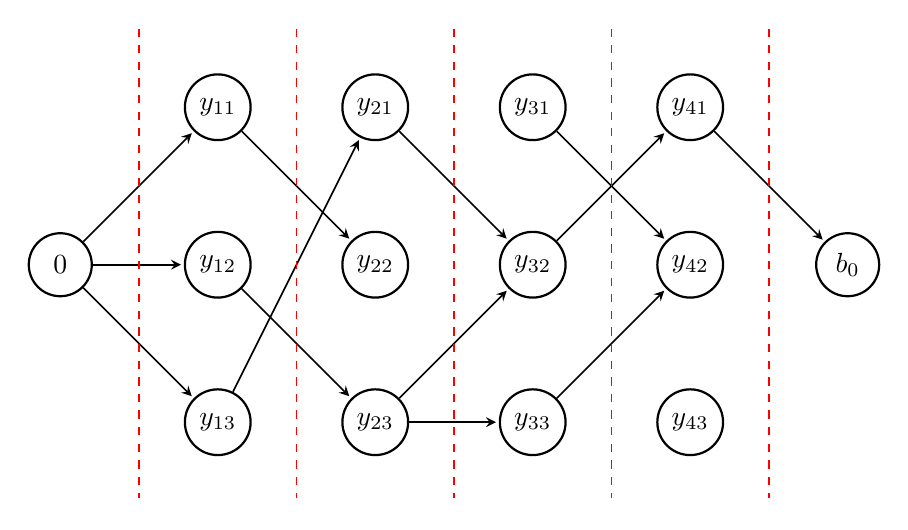
\begin{tikzpicture}[
            > = stealth, % arrow head style
            shorten > = 1pt, % don't touch arrow head to node
            auto,
            node distance = 3cm, % distance between nodes
            semithick % line style
        ]

        \tikzstyle{every state}=[
            draw = black,
            thick,
            fill = white,
            minimum size = 4mm
        ]

        \node[state, minimum size=0.8cm] (s) at (0,0) {$0$};
        
        \node[state] (w1) at (2,2)  {$y_{11}$};
        \node[state] (u1) at (2,0)  {$y_{12}$};
        \node[state] (v1) at (2,-2) {$y_{13}$};
        
        %\node (u2) at (4,0)  {$\sum_{i=1}^\ell A_ix^*$};
        \node[state] (w2) at (4,2)  {$y_{21}$};
        \node[state] (u2) at (4,0)  {$y_{22}$};
        \node[state] (v2) at (4,-2) {$y_{23}$};
        
        \node[state] (w3) at (6,2)  {$y_{31}$};
        \node[state] (u3) at (6,0)  {$y_{32}$};
        \node[state] (v3) at (6,-2) {$y_{33}$};
        
        \node[state] (w4) at (8,2)  {$y_{41}$};
        \node[state] (u4) at (8,0)  {$y_{42}$};
        \node[state] (v4) at (8,-2) {$y_{43}$};
        
        \node[state, minimum size=0.8cm] (f) at (10,0)  {$b_0$};
        
        \path[->] (s) edge node  {} (v1);
        \path[->] (v1) edge node {} (w2);
        \path[->] (w2) edge node {} (u3);
        \path[->] (u3) edge node {} (w4);
        \path[->] (w4) edge node {} (f);
    
        \path[->] (s) edge node  {} (w1);
        \path[->] (s) edge node  {} (u1);
        
        \path[->] (w1) edge node {} (u2);
        \path[->] (u1) edge node {} (v2);
        
        \path[->] (v2) edge node {} (u3);
        \path[->] (v2) edge node {} (v3);
        
        \path[->] (w3) edge node {} (u4);
        \path[->] (v3) edge node {} (u4);

        \draw[red, dashed] (1, 3) -- (1, -3);
        \draw[red, dashed] (3, 3) -- (3, -3);
        \draw[red, dashed] (5, 3) -- (5, -3);
        \draw[red, dashed] (7, 3) -- (7, -3);
        \draw[red, dashed] (9, 3) -- (9, -3);
        
        % \node (S1) at (2,-3.5) {$S_1$};
        % \node (S2) at (4,-3.5) {$S_2$};
        % \node (S3) at (6,-3.5) {$S_3$};
        % \node (S4) at (8,-3.5) {$S_4$};
    \end{tikzpicture}
    \end{center}
        
    \end{frame}
        \begin{frame}
        \frametitle{N-Fold, from RLR to optimum}
        \begin{block}{Correspondence}
            A longest path from $(0,0)$ to $(n,b_0)$ in G(V,E) corresponds to an optimal solution of the N-Fold integer program.
        \end{block}
        
        % \begin{block}{Space for graph plot}
        %     \vspace{2cm}
        % \end{block}
        
        % \textit{Proof:}\\
        % Every path from $(0,0)$ to $(n,b_0)$ corresponds to a feasible point verifying the proximity bound. The path cost corresponds to the objective function in this point so it's bounded by $c^tz^*$. 
        
        % \vspace{0.3cm}
        % The optimum $z^*$ corresponds to a path from $(0,0)$ to $(n,b_0)$. If not, we could find a feasible point improving $z^*$. This means that the longest path has as weight at least $c^tz^*$.
        
        % \vspace{0.3cm}
                \begin{center}
    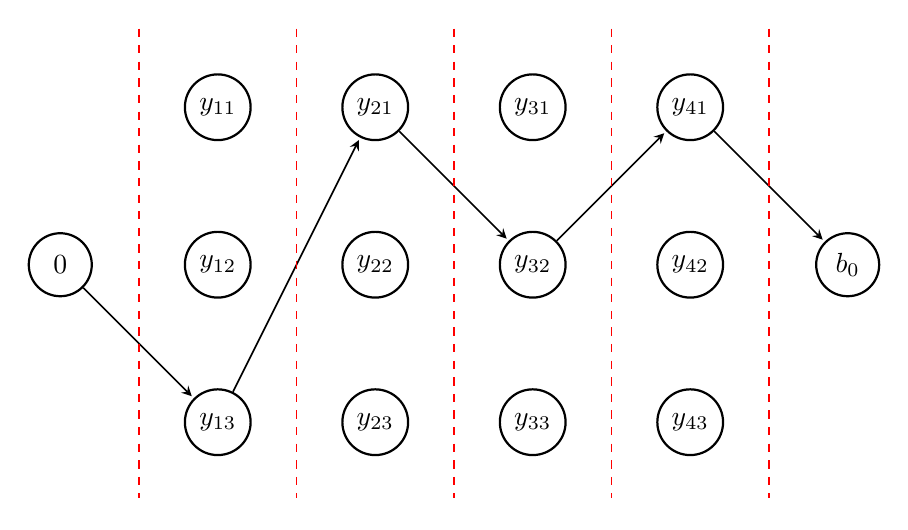
\begin{tikzpicture}[
            > = stealth, % arrow head style
            shorten > = 1pt, % don't touch arrow head to node
            auto,
            node distance = 3cm, % distance between nodes
            semithick % line style
        ]

        \tikzstyle{every state}=[
            draw = black,
            thick,
            fill = white,
            minimum size = 4mm
        ]

        \node[state, minimum size=0.8cm] (s) at (0,0) {$0$};
        
        \node[state] (w1) at (2,2)  {$y_{11}$};
        \node[state] (u1) at (2,0)  {$y_{12}$};
        \node[state] (v1) at (2,-2) {$y_{13}$};
        
        %\node (u2) at (4,0)  {$\sum_{i=1}^\ell A_ix^*$};
        \node[state] (w2) at (4,2)  {$y_{21}$};
        \node[state] (u2) at (4,0)  {$y_{22}$};
        \node[state] (v2) at (4,-2) {$y_{23}$};
        
        \node[state] (w3) at (6,2)  {$y_{31}$};
        \node[state] (u3) at (6,0)  {$y_{32}$};
        \node[state] (v3) at (6,-2) {$y_{33}$};
        
        \node[state] (w4) at (8,2)  {$y_{41}$};
        \node[state] (u4) at (8,0)  {$y_{42}$};
        \node[state] (v4) at (8,-2) {$y_{43}$};
        
        \node[state, minimum size=0.8cm] (f) at (10,0)  {$b_0$};
        
        \path[->] (s) edge node  {} (v1);
        \path[->] (v1) edge node {} (w2);
        \path[->] (w2) edge node {} (u3);
        \path[->] (u3) edge node {} (w4);
        \path[->] (w4) edge node {} (f);

        \draw[red, dashed] (1, 3) -- (1, -3);
        \draw[red, dashed] (3, 3) -- (3, -3);
        \draw[red, dashed] (5, 3) -- (5, -3);
        \draw[red, dashed] (7, 3) -- (7, -3);
        \draw[red, dashed] (9, 3) -- (9, -3);
        
        % \node (S1) at (2,-3.5) {$S_1$};
        % \node (S2) at (4,-3.5) {$S_2$};
        % \node (S3) at (6,-3.5) {$S_3$};
        % \node (S4) at (8,-3.5) {$S_4$};
    \end{tikzpicture}
    \end{center}
    \addtocounter{framenumber}{-1}
    \end{frame}
            \begin{frame}
        \frametitle{N-Fold, from RLR to optimum}
        \begin{block}{Correspondence}
            A longest path from $(0,0)$ to $(n,b_0)$ in G(V,E) corresponds to an optimal solution of the N-Fold integer program.
        \end{block}
        
        % \begin{block}{Space for graph plot}
        %     \vspace{2cm}
        % \end{block}
        
        % \textit{Proof:}\\
        % Every path from $(0,0)$ to $(n,b_0)$ corresponds to a feasible point verifying the proximity bound. The path cost corresponds to the objective function in this point so it's bounded by $c^tz^*$. 
        
        % \vspace{0.3cm}
        % The optimum $z^*$ corresponds to a path from $(0,0)$ to $(n,b_0)$. If not, we could find a feasible point improving $z^*$. This means that the longest path has as weight at least $c^tz^*$.
        
        % \vspace{0.3cm}
                \begin{center}
    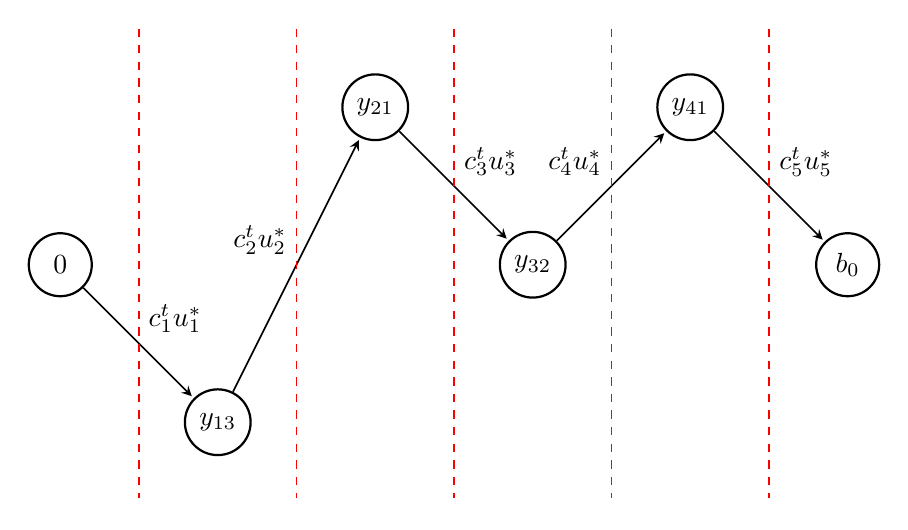
\begin{tikzpicture}[
            > = stealth, % arrow head style
            shorten > = 1pt, % don't touch arrow head to node
            auto,
            node distance = 3cm, % distance between nodes
            semithick % line style
        ]

        \tikzstyle{every state}=[
            draw = black,
            thick,
            fill = white,
            minimum size = 4mm
        ]

        \node[state, minimum size=0.8cm] (s) at (0,0) {$0$};
        
        %\node[state] (w1) at (2,2)  {$y_{11}$};
        %\node[state] (u1) at (2,0)  {$y_{12}$};
        \node[state] (v1) at (2,-2) {$y_{13}$};
        
        %\node (u2) at (4,0)  {$\sum_{i=1}^\ell A_ix^*$};
        \node[state] (w2) at (4,2)  {$y_{21}$};
        %\node[state] (u2) at (4,0)  {$y_{22}$};
        %\node[state] (v2) at (4,-2) {$y_{23}$};
        
        %\node[state] (w3) at (6,2)  {$y_{31}$};
        \node[state] (u3) at (6,0)  {$y_{32}$};
        %\node[state] (v3) at (6,-2) {$y_{33}$};
        
        \node[state] (w4) at (8,2)  {$y_{41}$};
        %\node[state] (u4) at (8,0)  {$y_{42}$};
        %\node[state] (v4) at (8,-2) {$y_{43}$};
        
        \node[state, minimum size=0.8cm] (f) at (10,0)  {$b_0$};
        
        \path[->] (s) edge node  {$c_1^tu_1^*$} (v1);
        \path[->] (v1) edge node {$c_2^tu_2^*$} (w2);
        \path[->] (w2) edge node {$c_3^tu_3^*$} (u3);
        \path[->] (u3) edge node {$c_4^tu_4^*$} (w4);
        \path[->] (w4) edge node {$c_5^tu_5^*$} (f);

        \draw[red, dashed] (1, 3) -- (1, -3);
        \draw[red, dashed] (3, 3) -- (3, -3);
        \draw[red, dashed] (5, 3) -- (5, -3);
        \draw[red, dashed] (7, 3) -- (7, -3);
        \draw[red, dashed] (9, 3) -- (9, -3);
        
        % \node (S1) at (2,-3.5) {$S_1$};
        % \node (S2) at (4,-3.5) {$S_2$};
        % \node (S3) at (6,-3.5) {$S_3$};
        % \node (S4) at (8,-3.5) {$S_4$};
    \end{tikzpicture}
    \end{center}
    \addtocounter{framenumber}{-1}
    \end{frame}
    \begin{frame}
    \frametitle{N-Fold, from RLR to optimum}
    \begin{block}{Correspondence}
    A longest path from $(0,0)$ to $(n,b_0)$ in G(V,E) corresponds to an optimal solution of the N-Fold integer program.
    \end{block}
    \begin{center}
    \begin{tikzpicture}[
            > = stealth, % arrow head style
            shorten > = 1pt, % don't touch arrow head to node
            auto,
            node distance = 3cm, % distance between nodes
            semithick % line style
        ]

        \tikzstyle{every state}=[
            draw = black,
            thick,
            fill = white,
            minimum size = 4mm
        ]

        \node[state, minimum size=0.8cm] (s) at (0,0) {$0$};
        
        %\node[state] (w1) at (2,2)  {$y_{11}$};
        %\node[state] (u1) at (2,0)  {$y_{12}$};
        \node (v1) at (2,-2) {$y_{1} = A_1u_1^*$};
        
        %\node (u2) at (4,0)  {$\sum_{i=1}^\ell A_ix^*$};
        \node (w2) at (4,2)  {$y_{2} = \sum_{i=1}^2A_iu_i^*$};
        %\node[state] (u2) at (4,0)  {$y_{22}$};
        %\node[state] (v2) at (4,-2) {$y_{23}$};
        
        %\node[state] (w3) at (6,2)  {$y_{31}$};
        \node (u3) at (6,0)  {$y_{3} = \sum_{i=1}^3A_iu_i^*$};
        %\node[state] (v3) at (6,-2) {$y_{33}$};
        
        \node (w4) at (8,2)  {$y_{4} = \sum_{i=1}^4A_iu_i^*$};
        %\node[state] (u4) at (8,0)  {$y_{42}$};
        %\node[state] (v4) at (8,-2) {$y_{43}$};
        
        \node[state, minimum size=0.8cm] (f) at (10,0)  {$b_0$};
        
        \path[->] (s) edge node  {} (v1);
        \path[->] (v1) edge node {} (w2);
        \path[->] (w2) edge node {} (u3);
        \path[->] (u3) edge node {} (w4);
        \path[->] (w4) edge node {} (f);

        \draw[red, dashed] (1, 3) -- (1, -3);
        %\draw[red, dashed] (3, 3) -- (3, -3);
        %\draw[red, dashed] (5, 3) -- (5, -3);
        %\draw[red, dashed] (7, 3) -- (7, -3);
        \draw[red, dashed] (9, 3) -- (9, -3);
        
        % \node (S1) at (2,-3.5) {$S_1$};
        % \node (S2) at (4,-3.5) {$S_2$};
        % \node (S3) at (6,-3.5) {$S_3$};
        % \node (S4) at (8,-3.5) {$S_4$};
    \end{tikzpicture}
    \end{center}
    \addtocounter{framenumber}{-1}
    \end{frame}
    
        \begin{frame}
    \frametitle{N-Fold, from RLR to optimum}
    \begin{block}{Correspondence}
    A longest path from $(0,0)$ to $(n,b_0)$ in G(V,E) corresponds to an optimal solution of the N-Fold integer program.
    \end{block}
    \begin{center}
    \begin{tikzpicture}[
            > = stealth, % arrow head style
            shorten > = 1pt, % don't touch arrow head to node
            auto,
            node distance = 3cm, % distance between nodes
            semithick % line style
        ]

        \tikzstyle{every state}=[
            draw = black,
            thick,
            fill = white,
            minimum size = 4mm
        ]

        \node[state, minimum size=0.8cm] (s) at (0,0) {$0$};
        
        %\node[state] (w1) at (2,2)  {$y_{11}$};
        %\node[state] (u1) at (2,0)  {$y_{12}$};
        \node (v1) at (2,-2) {$y_{1} = A_1z_1^*$};
        
        %\node (u2) at (4,0)  {$\sum_{i=1}^\ell A_ix^*$};
        \node (w2) at (4,2)  {$y_{2} = \sum_{i=1}^2A_iz_i^*$};
        %\node[state] (u2) at (4,0)  {$y_{22}$};
        %\node[state] (v2) at (4,-2) {$y_{23}$};
        
        %\node[state] (w3) at (6,2)  {$y_{31}$};
        \node (u3) at (6,0)  {$y_{3} = \sum_{i=1}^3A_iz_i^*$};
        %\node[state] (v3) at (6,-2) {$y_{33}$};
        
        \node (w4) at (8,2)  {$y_{4} = \sum_{i=1}^4A_iz_i^*$};
        %\node[state] (u4) at (8,0)  {$y_{42}$};
        %\node[state] (v4) at (8,-2) {$y_{43}$};
        
        \node[state, minimum size=0.8cm] (f) at (10,0)  {$b_0$};
        
        \path[->] (s) edge node  {} (v1);
        \path[->] (v1) edge node {} (w2);
        \path[->] (w2) edge node {} (u3);
        \path[->] (u3) edge node {} (w4);
        \path[->] (w4) edge node {} (f);

        \draw[red, dashed] (1, 3) -- (1, -3);
        %\draw[red, dashed] (3, 3) -- (3, -3);
        %\draw[red, dashed] (5, 3) -- (5, -3);
        %\draw[red, dashed] (7, 3) -- (7, -3);
        \draw[red, dashed] (9, 3) -- (9, -3);
        
        % \node (S1) at (2,-3.5) {$S_1$};
        % \node (S2) at (4,-3.5) {$S_2$};
        % \node (S3) at (6,-3.5) {$S_3$};
        % \node (S4) at (8,-3.5) {$S_4$};
    \end{tikzpicture}
    \end{center}
    \addtocounter{framenumber}{-1}
    \end{frame}
    
    % \begin{frame}
    % \begin{tikzpicture}[
    %         > = stealth, % arrow head style
    %         shorten > = 1pt, % don't touch arrow head to node
    %         auto,
    %         node distance = 3cm, % distance between nodes
    %         semithick % line style
    %     ]

    %     \tikzstyle{every state}=[
    %         draw = black,
    %         thick,
    %         fill = white,
    %         minimum size = 4mm
    %     ]

    %     \node[state] (s) {$(0,0)$};
    %     \node[state] (v1) [above right of=s] {$v_1$};
    %     %\node[state] (v2) [right of=s] {$v_2$};
    %     \node[state] (v3) [below right of=s] {$v_2$};
    %     \node[state] (t) [right of=v2] {$t$};

    %     \path[->] (s) edge node {18} (v1);
    %     %\path[->] (s) edge node {1} (v2);
    %     \path[->] (s) edge node {1} (v3);
    %     %\path[->] (v2) edge node {2} (v1);
    %     %\path[->] (v3) edge node {1} (v2);
    %     \path[->] (v1) edge node {20} (t);

    %     \draw[red, dashed] (1, 3) -- (1, -3);
    % \end{tikzpicture}
    % \end{frame}
    
    
    \begin{frame}
        \frametitle{N-Fold, from RLR to optimum}
        \begin{itemize}
            \item $|S_l| \leq (rs\Delta)^{O(r^2s)}$
            \item $|V| + |E| \leq O(n(rs\Delta)^{O(r^2s)})$
            \item The edge IP can be computed in time $t((r + s)\Delta)^{O(r + s)^2}$
            \item Longest path problem in a acyclic digraph can be solved in linear time.
        \end{itemize}
        \vspace{1cm}
        \begin{block}{N-Fold complexity}
            The N-Fold IP can be solved in time $nt(rs\Delta)^{O(r^2s + s^2)} + RLR$
        \end{block}
        [Cslovjecsek, Eisenbrand, Weismantel 2020]
    \end{frame}
    
    \section{References}
    \begin{frame}[allowframebreaks] % Interesting option!
        \frametitle{References}
        \nocite{*}
        \printbibliography
    \end{frame}

\end{document}

